%% History:
%% May 2019 Tomi Männistö, Antti-Pekka Tuovinen proofreading; 30 vs. 40 cr theses, etc.
%% May 2019 Tomi Männistö changed from babelbib to bibtex; Abstract page (and other pages as well) reformatting.
%% January–May 2019 several issues fixed by Niko Mäkitalo; long fields in abstract
%% March 2018 template file extended by Lea Kutvonen to exploit HYthesisML.cls.
%% Feb2018 This template file for the use of HYgraduML.cls was  modified by Veli Mäkinen from HY_fysiikka_LuKtemplate.tex
%% authored by Roope Halonen ja Tomi Vainio in 2017.
%% Some text is also inherited from engl_malli.tex versions by Kutvonen, Erkiö, Mäkelä, Verkamo, Kurhila, and
%% Nykänen, to accompany tktltiki.cls (by Puolakka 2002).


%% Follow comments to support use.

%%%%%%%%%%%%%%%%%%%%%%%%%%%%%%%%%%%%%%%%%%%%%%%%%%%%%%%%%
%% STEP 1: Choose options for MSc / BSc layout and your bibliographic style
%%%%%%%%%%%%%%%%%%%%%%%%%%%%%%%%%%%%%%%%%%%%%%%%%%%%%%%%%

%%  Language: 
%%      finnish, swedish, or english
%%  Pagination (use twoside by default)  
%%      oneside or twoside,
%%  Study programme / kind of report
%%      csm  = pro gradu in new Computer science MSc;
%%      cs = pro gradu in old Computer Science MSc;
%%      tkt = BSc thesis in new curricula;
%%      tktl= BSc thesis in old curricula;
%%  For MSc choose your line or track:
%%      (30 cr thesis, 2020 onwards, Master of Computer Science programme = csm)
%%      software-track-2020 = Software study track
%%      algorithms-track-2020 = Algorithms study track
%%      networking-track-2020 = Networking study track
%%
%%      (30 cr thesis, Master of Computer Science programme = csm)
%%      sw-track-2018 = Software Systems study track
%%      alko-track-2018 = Algorithms study track
%%      nodes-track-2018 = Networking and Services study track
%%
%%      (30 cr thesis, Master of Computer Science programme = csm)
%%      sw-line-2017 =  Software systems subprogramme
%%      alko-line-2017 = Algorithms, Data Analytics and Machine Learning subprogramme
%%      bio-line-2017 = Algorithmic Bioinformatics subprogramme
%%      nodes-line-2017 = Networking and Services subprogramme
%%
%%      (40 cr thesis, = cs)
%%      sw-line = Software Systems specialisation line 
%%      alko-line = Algorithms specialisation line
%%      bio-line = Algorithmic bioinformatics specialisation line
%%      nodes-line = Networking and Services specialisation line

\documentclass[finnish,twoside,censored,tkt,sw-line]{HYthesisML}


% In theses, open new chapters only at right page.
% For other types of documents, may ask "openany" in document.
\PassOptionsToClass{openright,twoside,a4paper}{report}
%\PassOptionsToClass{openany,twoside,a4paper}{report}

\usepackage{csquotes}
%%%%%%%%%%%%%%%%%%%%%%%%%%%%%%%%%%%%%%%%%%%%%%%%%%%%%%%%%
%% REFERENCES
%% Some notes on bibliography usage and options:
%% natbib -> you can use, e.g., \citep{} or \parencite{} for (Einstein, 1905); with APA \cite -> Einstein, 1905 without ()
%% maxcitenames=2 -> only 2 author names in text citations, if more -> et al. is used
%% maxbibnames=99 as no great need to suppress the biliography list in a thesis
%% for more information see biblatex package documentation, e.g., from https://ctan.org/pkg/biblatex 

%% Reference style: select one 
%% for APA = Harvard style = authoryear -> (Einstein, 1905) use:
%%\usepackage[style=authoryear,bibstyle=authoryear,backend=biber,natbib=true,maxnames=99,maxcitenames=2,giveninits=true,uniquename=init]{biblatex}
%% for numeric = Vancouver style -> [1] use:
\usepackage[style=numeric,bibstyle=numeric,backend=biber,natbib=true,maxbibnames=99,giveninits=true,uniquename=init]{biblatex}
%% for alpahbetic -> [Ein05] use:
%\usepackage[style=alphabetic,bibstyle=alphabetic,backend=biber,natbib=true,maxbibnames=99,giveninits=true,uniquename=init]{biblatex}
%

\addbibresource{bibliography.bib}
% in case you want the final delimiter between authors & -> (Einstein & Zweistein, 1905) 
% \renewcommand{\finalnamedelim}{ \& }
% List the authors in the Bibilipgraphy as Lastname F, Familyname G,
\DeclareNameAlias{sortname}{family-given}
% remove the punctuation between author names in Bibliography 
%\renewcommand{\revsdnamepunct}{ }


%% Block of definitions for fonts and packages for picture management.
%% In some systems, the figure packages may not be happy together.
%% Choose the ones you need.

%\usepackage[utf8]{inputenc} % For UTF8 support, in some systems. Use UTF8 when saving your file.

\usepackage{lmodern}         % Font package, again in some systems.
\usepackage{textcomp}        % Package for special symbols
\usepackage[pdftex]{color, graphicx} % For pdf output and jpg/png graphics
\usepackage{epsfig}
\usepackage{subfigure}
\usepackage[pdftex, plainpages=false]{hyperref} % For hyperlinks and pdf metadata
\usepackage{fancyhdr}        % For nicer page headers
\usepackage{tikz}            % For making vector graphics (hard to learn but powerful)
%\usepackage{wrapfig}        % For nice text-wrapping figures (use at own discretion)
\usepackage{amsmath, amssymb} % For better math

\singlespacing               %line spacing options; normally use single

\fussy
%\sloppy                      % sloppy and fussy commands can be used to avoid overlong text lines
% if you want to see which lines are too long or have too little stuff, comment out the following lines
% \overfullrule=1mm
% to see more info in the detailed log about under/overfull boxes...
% \showboxbreadth=50 
% \showboxdepth=50

\newcommand\todo[1]{\textcolor{red}{#1}}
\graphicspath{ {./kuvat/} }

%%%%%%%%%%%%%%%%%%%%%%%%%%%%%%%%%%%%%%%%%%%%%%%%%%%%%%%%%
%% STEP 2:
%%%%%%%%%%%%%%%%%%%%%%%%%%%%%%%%%%%%%%%%%%%%%%%%%%%%%%%%%
%% Set up personal information for the title page and the abstract form.
%% Replace parameters with your information.
\title{Moniasiakasjärjestelmän haasteet}

% TM: Contributors to template editors now listed in the beginning of the file in comments
\author{Felix Lindholm}
\date{\today}



% Set supervisors and examiners, use the titles according to the thesis language
% Prof. 
% Dr. or in Finnish toht. or tri or FT, TkT, Ph.D. or in Swedish... 
\supervisors{}
\examiners{}


\keywords{ulkoasu, tiivistelmä, lähdeluettelo}
\additionalinformation{\translate{\track}}

%% For seminar papers and such, cover page and abstract
%% requires these three basic items of information.
%% Label as needed and remove comment marks.
%%\level{Seminaariraportti}
%%\programme{Tietojenkäsittelytieteen andidaattiohjelma}
%%\subject{Seminaarisarjan nimi}

%% Replace classification terms with the ones that match your work. ACM
%% ACM Digital library provides a taxonomy and a tool for classification
%% in computer science. Use 1-3 paths, and use right arrows between the
%% about three levels in the path; each path requires a new line.

\classification{\protect{\ \\
\  General and reference $\rightarrow$ Document types  $\rightarrow$ Surveys and overviews\  \\
\  Applied computing  $\rightarrow$ Document management and text processing  $\rightarrow$ Document management $\rightarrow$ Text editing
}}

%% if you want to quote someone special. You can comment this line out and there will be nothing on the document.
%\quoting{Bachelor's degrees make pretty good placemats if you get them laminated.}{Jeph Jacques}


%% OPTIONAL STEP: Set up properties and metadata for the pdf file that pdfLaTeX makes.
%% Your name, work title, and keywords are recommended.
\hypersetup{
    unicode=true,           % to show non-Latin characters in Acrobat’s bookmarks
    pdftoolbar=true,        % show Acrobat’s toolbar?
    pdfmenubar=true,        % show Acrobat’s menu?
    pdffitwindow=false,     % window fit to page when opened
    pdfstartview={FitH},    % fits the width of the page to the window
    pdftitle={},            % title
    pdfauthor={},           % author
    pdfsubject={},          % subject of the document
    pdfcreator={},          % creator of the document
    pdfproducer={pdfLaTeX}, % producer of the document
    pdfkeywords={something} {something else}, % list of keywords for
    pdfnewwindow=true,      % links in new window
    colorlinks=true,        % false: boxed links; true: colored links
    linkcolor=black,        % color of internal links
    citecolor=black,        % color of links to bibliography
    filecolor=magenta,      % color of file links
    urlcolor=cyan           % color of external links
}

%%-----------------------------------------------------------------------------------

\begin{document}

% Generate title page.
\maketitle


%%%%%%%%%%%%%%%%%%%%%%%%%%%%%%%%%%%%%%%%%%%%%%%%%%%%%%%%%
%% STEP 3:
%%%%%%%%%%%%%%%%%%%%%%%%%%%%%%%%%%%%%%%%%%%%%%%%%%%%%%%%%
%% Write your abstract to be positioned here.
%% You can make several abstract pages (if you want it in different languages),
%% but you should also then redefine some of the above parameters in the proper
%% language as well, in between the abstract definitions.

\begin{abstract}

Tämä dokumentti on tarkoitettu Helsingin yliopiston tietojenkäsittelytieteen osaston opin\-näyt\-teiden ja harjoitustöiden ulkoasun ohjeeksi ja mallipohjaksi. Ohje soveltuu kanditutkielmiin, ohjelmistotuotantoprojekteihin, seminaareihin ja maisterintutkielmiin. Tämän ohjeen lisäksi on seurattava niitä ohjeita, jotka opastavat valitsemaan kuhunkin osioon tieteellisesti kiinnostavaa, syvällisesti pohdittua sisältöä.


Työn aihe luokitellaan  
ACM Computing Classification System (CCS) mukaisesti, 
ks.\ \url{https://www.acm.org/about-acm/class},
käyttäen komentoa \verb+\classification{}+. 
Käytä muutamaa termipolkua (1--3), jotka alkavat juuritermistä ja joissa polun tarkentuvat luokat erotetaan toisistaan oikealle osoittavalla nuolella.

\end{abstract}

\begin{otherlanguage}{english}
\begin{abstract}
Use this otherlanguage environment to write your abstract in another language if needed.

Topics are classified according to the ACM Computing Classification System
(CCS), see 
\url{https://www.acm.org/about-acm/class}:
check command \verb+\classification{}+. A small set of paths (1--3) should be used, starting from any top nodes
referred to bu the root term CCS leading to the leaf nodes. The elements
in the path are separated by right arrow, and emphasis of each element individually can be indicated
by the use of bold face for high importance or italics for intermediate
level. The combination of individual boldface terms may give the reader
additional insight. 
\end{abstract}
\end{otherlanguage}

% Place ToC
\newpage
\mytableofcontents
\mainmatter

%%%%%%%%%%%%%%%%%%%%%%%%%%%%%%%%%%%%%%%%%%%%%%%%%%%%%%%%%
%% STEP 4: Write the thesis.
%%%%%%%%%%%%%%%%%%%%%%%%%%%%%%%%%%%%%%%%%%%%%%%%%%%%%%%%%
%% Your actual text starts here. You shouldn't mess with the code above the line except
%% to change the parameters. Removing the abstract and ToC commands will mess up stuff.
%%
%% You may wish to include material to avoid browsing the definitions
%% above. Command \include{file} includes the file of name file.tex.
%% As a side effect, subsequent inclusions may force a page break.

% BSc instructions
\chapter{Johdanto}
Perinteisesti yritysten käyttämät toiminnanohjausjärjestelmät tai muut olennaiset ohjelmistot ovat olleet asennettuina asiakkaan omille laitteille, mutta nää ovat pikkuhiljaa alkaneet siirtymään pilviympäristöihin \cite{kaplan2007saas}. Tämän johdosta myös palveluiden palvelinkustannusten optimointi on noussut olennaiseksi kysymykseksi. Kun ohjelmisto onkin ajossa pilvipalvelussa perinteisen oman palvelinympäristön sijaan, on mahdollista tehostaa palvelinten käyttöastetta moniasiakasmallia hyödyntämällä \cite{momm2011qualitative}.

Moniasiakasjärjestelmää suunnitellessa on kuitenkin omat haasteensa, jotka voivat aiheuttaa suoria ja epäsuoria kustannuksia \cite{bezemer2010multi}. Tämän tutkielman tarkoituksena on pureutua näihin kysymyksiin ja selvittää millaisia haasteita moniasiakaspalveluissa on aiemmin havaittu ja miten näitä on ratkaistu. Tavoitteena on ymmärtää, millaisia kompromisseja asiakaskohtaisesta järjestelmästä moniasiakasmalliin siirtyessä on tehtävä, ja missä tilanteissa se on järkevää.

Moniasiakasjärjestelmät ovat nykyään huomattavasti yleistyneet \cite{kaplan2007saas}. Niiden haasteiden tutkiminen on kuitenkin edelleen mielenkiintoista, jotta voidaan tunnistaa tilanteet, joihin tällainen malli ei sovellu tai millaisissa tapauksissa asiakaskohtainen malli voi olla lopulta parempi ratkaisu. Vaikka moniasiakasmallin ja asiakaskohtaisten järjestelmien välillä vaihtaminen on jälkikäteen mahdollista, voi huomattavilta ylimääräisiltä kehityskustannuksilta \cite{momm2011qualitative} välttyä pohtimalla moniasiakasmallin haasteita ja hyötyjä jo toteutusvaiheessa.

Tässä tutkielmassa moniasiakasjärjestelmien haasteita selvitetään tutkimalla tapauksia tällaisista järjestelmistä, joista on kirjoitettu riittävän laaja ja luotettava kuvaus. Lisäksi moniasiakasjärjestelmän määrittelemiseksi ja aiheen pohjustamiseksi on käytetty aiemmin aiheesta kirjoitettuja artikkeleita. Aiheesta on aiemmin kirjoitettu yleisellä tasolla jonkin verran, mutta kuvauksia tällaisista järjestelmistä on niukasti saatavilla.

Toisessa luvussa määritellään moniasiakasjärjestelmä tämän tutkielman puitteissa, määrittämällä oleelliset piirteet, joissa se eroaa perinteisestä asiakaskohtaisesta järjestelmästä. Valittuja olennaisia piirteitä on taustoitettu aiheesta aiemmin kirjoitettujen artikkelien pohjalta. Lisäksi toisessa luvussa on kerrottu asiakaskohtaisista järjestelmistä ja syistä, miksi tällaisia järjestelmiä edelleen käytetään.

Kolmannessa luvussa esitellään tutkielmaan valitut tapaukset moniasiakasjärjestelmän toteutuksista, ja pureudutaan näissä järjestelmissä ilmeneviin haasteisiin ja ratkaisuihin. Jokaisesta tapauksesta on kirjoitettu oma kuvaus niistä tehtyjen artikkelien pohjalta. Neljännessä luvussa vertaillaan valittujen tapausten eroja ja yhtäläisyyksiä, ja tehdään johtopäätökset yleisimmin esiin nousseiden haasteiden ja ratkaisujen perusteella.

\chapter{Moniasiakasjärjestelmän määrittely}
Tässä luvussa tutkitaan asiakaskohtaisia järjestelmiä ja moniasiakasjärjestelmiä niiden vaihtoehtona. Käsittelen lyhyesti millaisia ohjelmistoja useimmiten toteutetaan asiakaskohtaisina järjestelminä, ja mitä hyötyjä sillä voi olla. Toisessa alaluvussa käsittelemme moniasiakasjärjestelmän piirteitä ja eroavaisuuksia asiakaskohtaisesta järjestelmästä, sekä määritelemme moniasiakasjärjestelmän käsitteen tämän tutkielman puitteissa.

\begin{figure}[h]
  \centering
  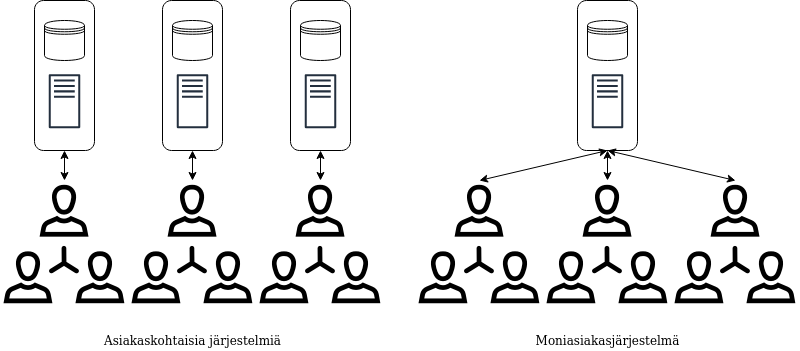
\includegraphics[width=16cm]{kuvat/yksi_vs_moni.png}
  \caption{Moniasiakasjärjestelmässä jokainen asiakasorganisaatio käyttää samoja järjestelmän instansseja.}
\end{figure}


\section{Asiakaskohtaiset järjestelmät}
Asiakaskohtaisina järjestelminä on perinteisesti kehitetty ainakin yrityksen liiketoiminnan hallintaan tarkoitettuja järjestelmiä, kuten toiminnanohjausjärjestelmiä ja asiakkuudenhallintajärjestelmiä \cite{stamelos2003estimating, kaplan2007saas}. Tällainen sovellus voi olla toteutettuna asiakkasyritykselle tilauksesta täysin heidän tarpeidensa mukaan tai yrityksen oman ohjelmistokehitystiimin toimesta. Molemmissa tapauksissa kustannusten arvioiminen on vaikeaa ja epäonnistuu usein \cite{stamelos2003estimating}. Kustannusten pienentämiseksi ja ennakoitavuuden parantamiseksi asiakaskohtaisia järjestelmiä on tilattu paljon myös sovelluspalveluntarjoajan kautta \cite{kaplan2007saas}.

Vaikka moniasiakasjärjestelminä toimivat ohjelmistopalvelut ovat yleistyneet, monet organisaatiot edelleen käyttävät ja toteuttavat asiakaskohtaisia järjestelmiä. Syitä olla siirtymättä valmiisiin ohjelmistopalveluihin ovat moninaisia, esimerkiksi riippumattomuus palveluntarjoajasta, räätälöidyn ratkaisun tarve ja erilaiset juridiset syyt \cite{janssen2011challenges}.

Toisaalta asiakaskohtainen järjestelmä voi olla myös valmiina tuotteena lisenssillä myytävä järjestelmä, jonka asiakasorganisaatio ostaa ja asentaa omalle laitteistolleen \cite{kinnunen2020yritysjarjestelmat}. Tällaisen mallin etuna asiakkaan näkökulmasta on pitkällä aikavälillä usein pienempi kokonaiskustannus. Lisäksi omalle laitteistolle asennettuun ohjelmistoon asiakas voi halutessaan tehdä lähes millaisia räätälöintejä tahansa, mutta tällaiset räätälöinnit saatta \todo{ASDF}

\section{Moniasiakasjärjestelmän oleellisia piirteitä}
Moniasiakasjärjestelmistä puhuttaessa voidaan viitata hyvinkin erilaisiin kokonaisuuksiin. Tässä luvussa määritellään moniasiakasjärjestelmä tämän tutkielman puitteissa ja tutkitaan, miten se poikkeaa asiakaskohtaisesta järjestelmästä. Bezmer ja Zaidman \cite{bezemer2010multi} määrittelevät moniasiakasjärjestelmän suoraviivaisesti ja selkeästi: Moniasiakasjärjestelmä sallii asiakkaiden jakaa sama laitteisto tarjoamalla käyttöön jaettu ohjelmiston ja tietokannan instanssi, samalla mahdollistaen ohjelman mukauttamisen asetuksilla omiin tarpeisiinsa.

Bezmer ja Zeidman on lisäksi nostanut esiin seuraavia oleellisia piirteitä moniasiakasjärjestelmistä:

\begin{enumerate}
  \item Järjestelmässä on asiakkaiden kesken jaetut fyysiset palvelimet.
  \item Järjestelmä on asiakaskohtaisesti muokattavissa käyttäjien tarpeiden mukaan.
  \item Järjestelmässä on asiakkaiden kesken jaetut tietokannat ja ohjelmiston ajossa olevat instanssit.
\end{enumerate}

Useimmat nykyaikaiset ohjelmistopalvelut täyttävät nämä piirteet jossain määrin. Määritelmän rajaamiseksi tässä tutkielmassa erottelemme vielä tavalliset monen käyttäjän palvelut moniasiakasjärjestelmistä olettamalla, että moniasiakasjärjestelmässä on useita organisaatioita, joista jokaisella voi olla useita käyttäjiä ja käyttäjäryhmiä.

\subsection{Jaetut palvelimet}
Kaikki asiakkaat käyttävät samaa fyysistä laitteistoa. Tämän avulla moniasiakasjärjestelmässä saavutetaan asiakaskohtaisia järjestelmiä parempi kustannustehokkuus. Kun kaikki asiakkaat jakavat saman laitteiston, saadaan käyttöaste paremmaksi. Tämä osaltaan aiheuttaa joitain haasteita, joita käsitellään myöhemmissä luvuissa.

Jaettuja palvelimia voidaan hyödyntää myös käyttämättä moniasiakasjärjestelmää, esim. ajamalla asiakaskohtaisia järjestelmiä virtualisoiduissa ympäristöissä. Tämä voi tapahtua joko asiakkaan omilla palvelimilla, tai pilvipalveluja hyödyntämällä. Näin voidaan saavuttaa merkittäviä hyötyjä asiakaskohtaisiin palvelimiin verrattuna, mutta virtualisoinnin aiheuttama resurssihukan takia hyötysuhdetta ei saada yhtä hyväksi kuin jaetuilla instansseilla.

\subsection{Jaetut tietokannat ja ohjelmiston ajossa olevat instanssit}
Jaetun fyysisen laitteiston lisäksi palvelimia ei ole jaettu asiakkaiden kesken esimerkiksi erillisillä virtualisoiduilla ympäristöillä. Virtualisoituihin ympäristöihin verrattuna tässä arkkitehtuurissa on etuna se, että se ei aiheuta samanlaista resurssihukkaa, kuin kokonaisten ympäristöjen virtualisointi \cite{huber2011evaluating}.

Erityisesti asiakkaiden kesken jaetut tietokannat vaativat ohjelmiston suunnittelun kannalta erityistä huomiota. Koska asiakkaiden data sijaitsee samassa tietokannassa ja samoissa tauluissa, täytyy tietojen näkyvyys asiakkaiden välillä ratkaista ohjelmiston tasolla.

Tietokannan jakaminen asiakkaiden välillä voidaan toteuttaa joko siten, että samassa tietokannassa on asiakaskohtaiset taulut, tai jakamalla tiedot rivikohtaisesti asiakkaiden välillä. Asiakaskohtaiset taulut ovat helppo tapa eriyttää data ja toteuttaa pääsynhallinta asiakkaiden tietojen välillä. Samalla tietokannan taulujen määrä kasvaa huomattavasti, joka aiheuttaa sen, ettei yhdellä tietokannalla voi palvella yhtä monta asiakasta kuin käyttämällä jaettuja tauluja \cite{chong2006multi}.

\subsection{Palvelun asiakaskohtainen muokattavuus}
Palvelun asiakaskohtainen muokattavuus on usein olennainen piirre moniasiakasjärjestelmässä, koska sillä on tarkoitus korvata asiakaskohtaiset asennukset, joissa tyypillisesti on tehty erilaisia räätälöintejä kullekin asiakkaalle. Koska kaikki asiakkaat käyttävät samaa instanssia ohjelmistosta, ei ohjelmakoodia muokkaamalla voida tehdä asiakaskohtaisia muutoksia. Ohjelmakoodissa täytyy siis jo suunnitteluvaiheessa ottaa huomioon riittävä sovelluksen muokattavuus, ja asiakkaiden täytyy voida muuttaa ohjelman toimintaa ajonaikaisesti.

Ohjelmiston muokattavuuden tarpeet voivat olla hyvin eritasoisia. Yksinkertaisimmillaan järjestelmässä riittää pienet ulkoasun muokkaukset, mutta monimutkaisissa tapauksissa käyttäjät voivat luoda täysin omiin tarpeisiinsa erilaisia tietomalleja. Useimmiten tarve on jotain tältä väliltä, esimerkiksi omien työvaiheiden määrittämistä toiminnanohjausjärjestelmässä.

\chapter{Tapauksia moniasiakasjärjestelmistä}
Moniasiakasjärjestelmistä yleisesti on kirjoitettu jonkin verran, mutta hyvin raportoituja toteutuksia on niukasti saatavilla. Tässä luvussa käsittelen löytämiäni riittävän hyvin kuvattuja järjestelmiä ja pyrin tiivistämään järjestelmän arkkitehtuurin kannalta olennaiset ratkaisut ja ongelmat joita niillä on ratkaistu. Tapauksiksi on valittu Force.com \cite{weissman2009design} ja IBM:n sähköisten sopimusten hallintajärjestelmä \cite{kwok2008software}, sekä ScrewTurn Wikin \cite{bezemer2010challenges} ja Codename ohjelmiston \cite{bezemer2010enabling} muunnokset moniasiakasjärejestelmiksi.


\section{Force.com}
Force.com on SalesForce-yrityksen alusta, jota yli 50 000 organisaatiota käyttää oman ohjelmistopalvelunsa kehittämiseen. Alusta on moniasiakasjärjestelmäksi rakennettu, eli kaikki asiakkaat jakavat saman alusta, ilman erillisiä asiakaskohtaisia laitteistoja, tietokantoja tai muita ohjelmistoja. Weissman ja Bobrowski ovat kirjoittaneet kattavan kuvauksen \cite{weissman2009design} järjestelmän toteutuksesta.

Force.comin arkkitehtuuri on poikkeava normaalin ohjelmistopalvelun tavanomaisesta arkkitehtuurista, koska se on alusta, jossa samaan jaettuun järjestelmään voidaan rakentaa useita täysin erityyppisiä palveluja. Tämän takia alusta määrittelee kaiken metatietojen avulla. Esimerkiksi käyttäjän luodessa uusi taulu palveluunsa, järjestelmä luo tämän uuden taulun kuvauksen metatietona, jolla mallinnetaan halutunlainen virtuaalinen tietokantataulu kaikkien jakamaan hyvin geneeriseen tietokantamalliin. Virtuaalinen tietokantataulu tulkitaan ajonaikaisesti ja siihen tehdyt tietokantakyselyt muutetaan muotoon, jolla tiedot voidaan hakea hyvin joustavasti muotoillusta asiakkaiden kesken jaetusta tietokannasta.

Tällaisen erittäin joustavan tietokantarakenteen takia tavanomaisten tietokantaindeksien tekeminen kyselyjen optimoimiseksi ei ole mahdollista. Koska Force.comin tietokantataulun sarakkeet eivät ole kiinteästi tyypitetty, joudutaan asia ratkaisemaan toisin. Tätä varten järjestelmässä on oma taulu indekseille, jossa tieto on tyypitettynä ja se on indeksoitu. Tätä taulua hyödynnetään tietokantakyselyjen optimoimiseksi, kun käyttäjä hakee dataa tietokannasta. Lisäksi tietokantahakujen tehostamiseksi data on osioitu kannassa asiakastunnisteen perusteella.



\section{IBM:n sähköisten sopimusten hallintajärjestelmä}
Kwok ym. \cite{kwok2008software} kuvailevat IBM:n tutkimusryhmän kokeilua toteuttaa sähköisten sopimusten hallinnointijärjestelmä moniasiakasjärjestelmänä suunnitelluksi palveluksi. Raportin kirjoituksen aikaan 2008 palvelua oli pilotoitu yli 10 organisaatiolle ja yli 300 käyttäjälle, jotka kaikki jakavat samat resurssit. Tutkimusryhmän mukaan vastaava palvelut on perinteisesti toteutettu asiakaskohtaisina järjestelminä, joiden kustannukset tällaisina ovat niin suuret, ettei pienillä yrityksillä ole niihin varaa.

Ohjelmistossa on toteutettu erillinen autentikaatiopalvelu (Security services), joka merkitsee kunkin sisäänkirjautuneen käyttäjän asiakaskohtaisella tunnisteella. Tältä palvelulta ohjelmiston muut moduulit hakevat käyttäjälle tunnisteen, jonka perusteella palvelu mukautetaan ja näytettävät tiedot valitaan. Asiakaskohtaisia ohjelmiston mukautuksia hallitaan ja säädetään ohjelmiston metatietopalvelussa (Metadata services). Näillä molemmilla palveluilla on omat erilliset tietokannat (käyttäjätietojen tietokanta ja asiakkaan metatietojen tietokanta).

Käyttäjien sisäänkirjautuminen on järjestelmässä toteutettu keskitetyn autentikointipalvelun avulla. Tämä ratkaisu on helppo toteuttaa, koska se ei vaadi mitään asiakaskohtaista osuutta, mutta samasta syystä integraatio asiakkaan jo olemassa oleviin järjestelmiin on haasteellinen, eikä sitä ole tässä järjestelmässä toteutettukaan. Käyttäjä siis joutuu aina erikseen kirjautumaan tähän palveluun, eikä saumatonta kokemusta asiakkaan muiden järjestelmien välillä voida saavuttaa.

Käyttäjäkohtaista muokattavuutta varten järjestelmän tietokantamalliin on suunniteltu rakenne, johon voidaan tehdä joustavasti lisäyksiä määrittäen tarvittaville lisätiedoille tietokannassa oma rivikohtainen tyyppi ja tunniste. Mukautettava rakenne monimutkaistaa tietokantakyselyjä ja tekee niiden tehostamisen indeksien avulla haastavammaksi.

Järjestelmässä on toteutettu erillinen moduuli asiakkaiden käytön seurantaan. Tämän avulla määritellään, kuinka paljon asiakkaita laskutetaan, mutta myös varmistetaan, että ohjelmiston tehokkuus pysyy vaaditulla tasolla. Raportissa ei ole käsitellä juurikaan järjestelmän tehokkuuden optimointia tai skaalausratkaisuja. Toisaalta raportin aikaan palvelun käyttäjämäärät ovat vielä olleet maltillisia, eikä skaalaus ole välttämättä ole ollut tarpeellista.

\section{ScrewTurn Wiki}
ScrewTurn Wiki on avoimen lähdekoodin ohjelmisto, jonka muuntamisesta moniasiakasjärjestelmäksi on tehty raportti osana tutkimusta \cite{bezemer2010challenges}. Raportissa on käsitelty tarvittavat muutokset autentikaatioon ja tietokantaan, sekä moniasiakasjärjestelmänä palvelun mukautettavuuden toteutus.

Käyttäjien tunnistaminen tapahtuu erillisellä Kerberos-protokollaa hyödyntävällä palvelulla. Tältä palvelulta saatavassa tunnisteessa voidaan tallentaa kaikki tarvittava tieto, jolla käyttäjän asiakkuus voidaan varmistaa. Lisäksi järjestelmässä on autentikaatiomoduuli, joka jokaisen palveluun tehtävän kyselyn yhteydessä tunnistaa käyttäjän asiakkuuden.

Järjestelmän muokattavuutta ei tässä tapauksessa toteutettu kattavasti. Joidenkin asetusten käsitteleminen integroitiin alkuperäisestä toteutuksesta käyttämään tätä varten kehitettyjä kirjastoja, jotka vastaavat palvelun mukautuksesta. Myös tietokanta on muunnettu moniasiakkuusmallia tukevaksi hyvin pienin muutoksin. Tietokantaa varten on toteutettu abstraktiotaso, joka muuntaa kaikki tietokantakyselyt suodattamaan tulokset tunnistautumispalvelun antaman asiakastunnisteen perusteella.

\section{Exact Codename}
Exact Codename on Exact nimisen hollantilaisen ohjelmistoyrityksen kehitysprojekti, josta Bezemer ja Zaidman ovat tehneet ja raportoineet muunnoksen moniasiakasjärjestelmäksi \cite{bezemer2010enabling}. Codename on siis alunperin suunniteltu asiakaskohtaiseksi järjestelmäksi, mutta tutkimusprojektina muunnettu moniasiakasjärjestelmäksi minimaalisin muutoksin. Lähestyminen on siis samankaltainen kuin ScrewTurn Wikin tapauksessa, mutta siitä poiketen Codename on kaupallinen sovellus. Moniasiakasjärjestelmäksi muunnetun järjestelmän nimi tutkimusessa oli $Codename^{MT}$.

$Codename^{MT}$ liitettiin Exactin keskitettyyn tunnistautumisjärjestelmään, ja Codenamen käyttäjäobjektiin lisättiin asiakkuuden tunniste TenantID. Järjestelmän arkkitehtuurin ansiosta TenantID oli tällä tavoin käytettävissä järjestelmän kaikissa osissa, ja sitä voitiin hyödyntää käyttäjän näkemän tiedon rajoittamiseksi. Tämän toteuttamiseksi tietokantaan lisättiin tauluille määritelmä siitä, onko kyseinen taulu asiakaskohtainen vai jaettu. Asiakaskohtaisiin tauluihin lisättiin lisäksi sarake asiakastunnisteelle, jonka mukaan käyttäjille näytettävä data rajataan asiakaskohtaisesti suodattamalla kaikkia tietokantahakuja sen mukaan.

Järjestelmän mukautettavuuden toteutus jäi tutkimuksessa vajavaiseksi. Järjestelmään toteutettiin .NET-ohjelmistokehyksen valmiilla työkaluilla ulkoasun teemojen muokkaus asiakaskohtaisesti, sekä asiakaskohtaisten tiedostojen hallinta. Järjestelmän työnkulun asiakaskohtainen muokattavuus tunnistettiin olennaiseksi ja tutkimusta varten se suunniteltiin, mutta toteutus jäi sen osalta uupumaan.

Codenamen muunnos moniasiakasjärjestelmäksi onnistui vain noin 100 rivin lisäyksellä lähdekoodiin, ja aikaa tähän kului vain viisi päivää. Lisäksi kehittäjille näkyvä muutos järjestelmässä on hyvin pieni. Muunnoksessa ei tarvinnut muuttaa mitään olemassa olevia järjestelmän kannalta oleellisia ominaisuuksia, eikä se näy loppukäyttäjälle mitenkään.

\chapter{Johtopäätökset}

Tässä luvussa vertaillaan tutkittaviksi valittuja moniasiakasjärjestelmätoteutuksia. Olennaisiksi seikoiksi asiakaskohtaisiin ohjelmistoihin verrattuna olen valinnut seuraavat tekijät: tehokkuus, skaalaus, tietoturva ja ohjelmakoodin monimutkaistuminen. Koska kaksi neljästä valitusta tapauksesta oli muunnoksia asiakaskohtaisesta järjestelmästä moniasiakasjärjestelmäksi, viimeinen alaluku käsittelee vielä järjestelmän muunnosta omana haasteenaan.

\section{Tehokkuus}
Koska jokaisen asiakkaan käyttäjät käyttävät ohjelmiston samaa instanssia, vaikuttaa heidän toimintansa järjestelmässä toisiinsa. Yhden asiakkaan aiheuttaessa ongelmatilanteen järjestelmään, voivat kaikkien asiakkaiden järjestelmät olla poissa käytöstä. Tästä syystä on erityisen oleellista, että käyttäjä ei pysty tekemään sellaista toimenpidettä järjestelmässä, jonka tehokkuus on niin huono, että se vaikuttaa muiden asiakkaiden käyttökokemukseen.

Moniasiakasjärjestelmien tehokkuudessa on oleellista panostaa tietokantakyselyiden tehokkuuteen, kun asiakasmäärät kasvavat suuremmiksi. Koska kaikkien asiakkaiden tiedot sijaitsee samoissa tietokantatauluissa, täytyy tietojen indeksointi tehdä järkevästi. Asiakastunnisteelle tehdään kaikissa tauluissa indeksit siten, ettei tietokantahakujen tehokkuus kärsi vaikka datamäärä on huomattavan suuri asiakaskohtaiseen tietokantaan verrattuna. Lisäksi tietokantahakuja voidaan optimoida tietokannan osioinnilla asiakkuustunnisteen perusteella, kuten Force.com palvelussa \cite{weissman2009design}. Toisaalta järjestelmän käytön monitoroinnin näkymä voi olla tehokkuuden tarkkailua varten hyödyllinen, kuten IBM:n tutkimusryhmä \cite{kwok2008software} kertoo.

Force.com ja IBM:n järjestelmän tehokkuuden optimoinnissa olennainen osa on tietokantakyselyiden optimointi moniasiakasmallia tukevalla tavalla. ScrewTurn Wikin kohdalla tehokkuutta varten ei toisaalta tehty vielä minkäänlaisia toimenpiteitä, luultavasti koska sitä ei ole testattu vielä raportin aikana suuremmilla käyttäjämäärillä.

\section{Skaalaus}
Moniasiakasjärjestelmän skaalaus on teknisesti asiakaskohtaisia asennuksia yksinkertaisempaa, koska järjestelmästä on vain yksi asennus, eikä skaalausta tarvitse tehdä jokaisen asiakkaan kohdalla erikseen. Toisaalta koska moniasiakasjärjestelmässä käyttäjien määrä moninkertaistuu asiakaskohtaiseen asennukseen verrattuna, ajaudutaan nopeammin tilanteeseen, jossa pelkkä palvelimen tehon lisäys ei enää riitä, vaan joudutaan ajamaan ohjelmistoa usealla palvelimella, joiden välillä kuormaa jaetaan.

IBM:n tutkimusryhmä \cite{kwok2008software} kertoo suunnittelevansa skaalauksen tarkempaa tutkimista vaihtamalla ohjelmisto tehokkaammille palvelimille, ajamalla ohjelmistosta useampaa instanssia samanaikaisesti, ja tehostamalla tietokannan toimintaa jakamalla se pienempiin segmentteihin. Force.comin tärkeäksi pullonkaulaksi mainitaan \cite{weissman2009design} metadatan lukeminen ohjelmistossa, koska kaikki asiakaskohtainen muokattavuus toteutetaan näiden avulla. Jotta järjestelmä skaalautuisi, metadatoja säilötään muistissa pidettävään välimuistiin. Bezmer ja Zaidman \cite{bezemer2010challenges} mainitsevat oman lähtökohtansa huomioivan skaalauksen siten, että kaikki ohjelmiston komponentit on toteutettu erillisinä irrallaan skaalattavina palveluina.

\section{Tietoturva}
Asiakaskohtaisessa asennuksessa voidaan tehdä erilaisia toimenpiteitä tietoturvan parantamiseksi, jotka moniasiakasjärjestelmässä ei ole mahdollista. Asiakaskohtaista järjestelmää voidaan esimerkiksi ajaa kokonaan asiakkaan omassa lähiverkossa, ilman että se on lainkaan yhteydessä julkiseen internetiin. Vaikka järjestelmä olisi julkisessa internetissä, sinne pääsy voidaan rajata eri tavoin vain kyseiselle asiakkaalle.

Moniasiakasjärjestelmässä kehittäjät joutuvat myös huolehtimaan, että asiakkaalla on pääsy vain omaan dataansa, koska kaikkien asiakkaiden data on sijoitettu samaan tietokantaan. Yleisesti tämä ongelma ratkaistaan siten, että asiakaskohtainen pääsynhallinta on sisäänrakennettu sovellukseen riittävän vahvasti. Kaikella tiedolla tietokannassa on siis asiakkaan tunniste, ja ohjelmistossa ei tietokantakyselyjä ei voi tehdä, ilman että kaikkiin kyselyihin on liitetty asiakkaan tunniste sisäänkirjautuneen käyttäjän perusteella.

Tietoturvan kannalta kaikissa tutkituissa tapauksissa on pääpiirteittäin samanlainen ratkaisu. Käyttäjien pääsynhallintaan ja tunnistautumiseen on erillinen palvelu, joka määrittelee käyttäjälle asiakkuustunnisteen. Tämä asiakkuustunniste liitetään järjestelmässä kaikkiin toimenpiteisiin, joita käyttäjä tekee, ja tietokantakyselyihin on toteutettu riittävä abstraktio, jolla kyselyitä ei ole mahdollista tehdä ilman asiakastunnistetta.

Tietoturvakompromissi joka moniasiakasympäristöissä ei ole ratkaistavissa kuten asiakaskohtaisessa kohtaisissa järjestelmissä, on kohdistetun hyökkäyksen mahdollisuus vaarantaa kaikkien asiakkaiden data kerralla. Toisin sanoen, jos hyökkääjä tahtoo päästä tietyn asiakkaan tietoihin käsiksi, onnistuessaan hän saa samalla kaikkien asiakkaiden tiedot. Tämän estämiseksi on asiakkailla väistämättä oltava vähintäänkin omat asiakaskohtaiset tietokannat.

\section{Ohjelmakoodin monimutkaistuminen}

\todo{ekan lauseen sanajärjestys} Koska moniasiakasjärjestelmässä monia asioita, jotka ennen pystyttiin huomioimaan muilla tavoin, joudutaan nyt tekemään ajonaikaisesti ohjelmakoodissa, on se kehittäjille väistämättä monimutkaisempi. Tämän takia vaikka palvelinten ylläpidon puolelta työmäärä yksinkertaistuu ja vähenee, kehitystiimillä työtä on enemmän ja se on haastavampaa.

Eniten monimutkaisuutta aiheuttava tekijä moniasiakasjärjestelmissä on asiakaskohtainen muokattavuus. Koska tutkituissa tapauksissa asiakaskohtainen muokattavuus on toteutettu hyvin eri määrin, myös ohjelmakoodin ja järjestelmän arkkitehtuurin monimutkaisuus on tapausten välillä hyvin eritasoista.

Koska Force.com on alusta, jolle voi rakentaa hyvin vapaasti omanlaisensa ohjelmistopalvelun, on sen toiminnallisuus täysin käyttäjän määriteltävissä. Tämän takia myös ohjelmistossa on paljon monimutkaisia osia. Muihin järjestelmiin verrattaessa mielenkiintoista on tietokannan rakenne, joka sallii käyttäjän määritellä minkälaisen tahansa tietokantamallin. Tämä vaatii järjestelmältä paljon abstraktiota ja optimointia tietokannan päälle.

IBM:n digitaalisten sopimusten hallintajärjestelmässä käyttäjä pystyy tekemään erilaisia polkuja sopimusten hallinnointiin, ja lisäämään tietokantaan asiakaskohtaisia tietoja. Myös IBM:n järjestelmässä on tietokantaan siis toteutettu joustava osa, jolla asiakas voi lisätä omia tietorakenteita, mutta tätä ei ole toteutettu yhtä laajaksi kuin Force.comissa, eikä järjestelmässä voi tehdä täysin mielivaltaista tietokantamallia.

ScrewTurn Wikin moniasiakasjärjestelmän toteutus taas on toteutettu minimaalisin muutoksin alkuperäisestä järjestelmästä. Näin se ei ole paljon yhden asiakkaan asennusta monimutkaisempi, mutta myös vain hyvin rajallisesti muokattavissa.

Järjestelmän suunnittelijan kannalta on siis olennaista miettiä, kuinka paljon asiakkaan on voitava muokata ohjelmistoa omaan tarpeeseensa, ja miten tämä muokattavuus on helpoin toteuttaa. Jos käyttäjät hyötyvät monimutkaisista asiakaskohtaisista mukautuksista ja integraatioista paljon, voi olla tehokkaampaa ylläpitää ohjelmistosta asiakaskohtaisia versioita. Toisaalta useissa tapauksissa käyttäjien muokkaustarpeet voivat olla hyvin yksinkertaisia, ja asiakaskohtainen muokattavuus on tällöin helppo toteuttaa ajonaikaisesti.

\section{Järjestelmän muunnos}

Valituista tapauksista $Codename^{MT}$ ja ScrewTurn Wiki olivat muunnoksia asiakaskohtaisesta järjestelmästä moniasiakasjärjestelmäksi. Erityisesti $Codename^{MT}$ tapauksessa tarkoituksena oli tehdä muunnos minimaalisilla muutoksillä järjestelmän lähdekoodiin. Molemmissa tapauksissa asiakaskohtainen muokattavuus toteutettiin  vain pienimuotoisesti. Tapauksien perusteella voidaan kuitenkin osoittaa, että muunnos moniasiakasjärjestelmään jälkikäteen on mahdollista toteuttaa jopa kohtuullisen vaivattomasti. Suurin vaikuttava tekijä muunnoksen monimutkaisuuteen vaikuttaa olevan asiakaskohtaisen muokattavuuden toteutuksen laajuus.

Molemmissa tapauksissa pääsynhallinta dataan muutettiin asiakaskohtaiseksi lisäämällä tauluihin sarake asiakkuustunnisteelle, ja toteuttamalla erillinen moduuli tietokantakyselyjen muuttamiseksi. Tämän moduulin tehtävä on käsitellä kaikkia tietokantakyselyjä siten, että ne suodatetaan asiakkuustunnisteen perusteella käsittelemään vain tietyn asiakkaan dataa. Tällä tavoin toteutettuna muutos vaikuttaa erittäin vähän ohjelmistokehittäjien työhön, koska suodatus on abstraktoitu ohjelmakoodin seasta omaksi moduulikseen. Näin kehittäjien on myös vaikeampi tehdä virheitä, kun suodatus koskaa automaattisesti kaikkia tietokantakyselyjä.

\chapter{Yhteenveto}
Tutkielmassa selvitettiin moniasiakasjärjestelmän eroavaisuuksia perinteiseen asiakaskohtaiseen järjestelmään, ja erityisesti moniasiakasmallin haasteita. Etsin hyvin dokumentoituja tapauksia tällaisista järjestelmistä, ja vertailin miten näissä on ratkaistu moniasiakasjärjestelmän aiheuttamia haasteita. Tutkielmassa on esimerkkitapausten lisäksi käytetty aiheesta aiemmin kirjoitettuja artikkeleita ongelman taustoittamiseksi ja moniasiakasjärjestelmän määrittelemiseksi.

Moniasiakasjärjestelmämalli on monille palveluntarjoajille hyvä vaihtoehto, jolla palvelun kustannustehokkuutta voidaan parantaa. Suurin osa moniasiakasjärjestelmän haasteista on ratkaistavissa siten, että ainoana kompromissina asiakaskohtaiseen järjestelmään on ohjelmiston monimutkaistuminen. Ohjelmiston monimutkaistuminen kuitenkin on useissa tapauksissa varmasti kannattava ratkaisu moniasiakasjärjestelmän tarjoamien etujen takia. Tämän tutkielman puitteissa ainoa esiin noussut ratkaisematon haaste on asiakkaan parhaan mahdollisen tietoturvan saavuttaminen. Asiakaskohtaisessa asennuksessa väistämättä voidaan tehdä vahvempi tietoturva, rajaamalla järjestelmään pääsyä vain asiakasorganisaatiolle. Lisäksi toiseen asiakkaaseen kohdennettu isku ei vaaranna kaikkien muiden tietoja asiakaskohtaisessa ympäristössä.

Järjestelmän toteutusta suunnitellessa vaaditun asiakaskohtaisen muokattavuuden määritteleminen on ehkä yksittäisenä tekijänä oleellisin huomioitava. Mitä vapaammin asiakkaan muokattavissa järjestelmä on, sitä monimutkaisempia ratkaisuja joudutaan toteuttamaan. Yksinkertaisimmillaan mukautettavuus voi olla ennalta määritettyjä asetuksia tietokannassa, ja monimutkaisimmillaan tietokantamalli, jossa käyttäjä pystyy määrittämään mielivaltaisesti virtuaalisia tauluja järjestelmään.

\todo{tähän viel kappale muunnoksesta ehkä??}

%
\chapter{Introduction}


In all writing for publication, the writer's freedom of creation and expression are limited by a number of guidelines and specific regulations.

At best, a familiar set of regulations shared by reader and writer can create a kind of support network that allows the message to be relayed without distortion. It will be easier for readers to find 
the pertinent contents in a piece of writing if its layout and structure are the same as they are used to. This also applies to writers. When writers follow a set presentation model, 
they do not have to waste time on considerations that are secondary to the work itself, but they can concentrate on polishing the contents of the text. This means that it is a good 
idea to practice following the rules for the layout, though you may think you know how to select a better way to present your work.

This is a guide for the layout and structure of theses and essays at the Department of Computer Science at the University of Helsinki. It is thus applicable to the course 
Scientific Writing, the software engineering projects, seminars, and MSc theses. (This is an updated version of 
the previous guide written by the course lecturers \citep{erkio01, erkiomakela96, erkio94, verkamo92}.)

The \LaTeX\ guide and \LaTeX\ style that has been  published on the department's web site can be used as support for this guide.


\chapter{Structure}

Let us start by looking at the sections expected to be in a scientific text. Keep in mind that the same expectations go for all kinds of technical writing.
However, this document in itself, is not a scientific or a research
text, so there will be content lacks in terms of research question
setting in the introduction and evaluative material in the last sections.

\section{Abstract or summary}
%\enlargethispage{5mm}


The summary page contains the following elements: the bibliographical data of the work, an abstract, topic classification, 
and the key words. The bibliographical data consists of title, name of the author, place of publication, date of publication, and number of pages.

The abstract should be short, generally one paragraph (100 words maximum) explaining the main contents of the work: topic, methodology and results.


 Topics are classified according to the ACM Computing Classification System
(CCS). A small set of paths (1-3) should be used, starting from any top nodes
referred to bu the root term CCS leading to the leaf nodes. The elements
in the path are separated by right arrow, and emphasis of each element individually can be indicated
by the use of bold face for high importance or italics for intermediate
level. The combination of individual boldface terms may give the reader
additional insight. 

\section{Introduction}


The purpose of the introduction is to introduce the goals of the work in general terms. Describe topic, 
methodology and results (as in the abstract, but expand it).
In order to provide the reader a good starting point for
interpretations, it is good to start the introduction by
contextualisation of the challenges and solutions to be discussed. For
example, why a certain domain has a particular challenge and who are
intended to benefit from the solutions proposed.

The length of the introduction depends on the length of the whole work. A few pages of text does not need a 
separate introduction, since it is an expanded summary in itself. The introduction to a 10-page text can 
be 1--1.5 pages long. For a 50--70-page MSc thesis, a 2--4-page introduction seems reasonable.

The introduction should shortly describe the problem field of the whole work, the plot, and the conclusions, 
in general terms. After reading it, the reader may decide whether to go deeper into the topic by reading the whole text.


\section{Topic chapters}

The nature of the matter at hand determines how the topic chapters are disposed.
In order to guide the reader, it is a good idea to start each main chapter with a short paragraph 
on what the main topic of the chapter is and how it progresses from one sub-chapter to the
next. Especially relevant is to express how concepts, challenges,
solutions and research steps are bound together. There should be enough
guidance for the reader to allow expectation of the right storyline.


Basic rule for easy to follow text is to use the natural emphasis of the
text structure to support the content matter key concepts and thought
processes. This means using openings of sectiosn and text paragraphs for
key arguments and information moves, while the internal parts of
paragraps are filled with supporting aspects that those less familiar
with the topic area need. Those with better background knoweldge can
quickly skim trhough the text without loosing any essential arguments.

Each author has his or her personal ryhtm in the text, which is visible
for the reader as the length of text paragraphs and complexity of
thought chains within. A good policy is to take only one information
move or transition per paragraph. This way the text stays easy to follow.

Signs of problems with the disposition of the text are easily seen in texts
with only one sub-chapter, or with more than two chapter levels (main and sub-chapters). There may be justifiable reasons to use three-level 
headings in some technical documents. Single sentence text paragraphs
are also to be avoided.



%\pagebreak
\section{Reference usage}


Relevant learning targets include superficial knowledge of several
citation styles and capability (and willingness) to follow a given
style and ordering of entires and bibliographical details in the list of references.
These aspects are essential as the approval of a PhD manuscript or
journal article may depend on them.

Disregard of which style you use, 
references are always placed inside sentences.  This means that e.g. a separate reference at the end of a paragraph would be inappropriate.

The structure of the text must clearly show what the reference relates to.  At the same time, it 
shows how long a piece of the text that the reference relates to.

Efficient positions for citations are right after the introduction
(definition) of a concept, a methods or such, or in the end of a claim
from the reference material. Furthermore, if quoting verbatime one must
use citation marks.

The text structures and wordings, in addition to the location of
ciations must clearly express whether claims or arguments are 
authors' own, or if they come from the contribution of others. Thus is
is of bad style to open a section by listing the citations on which the
section is based on. Such method can further indicate more serious
problems like following reference material as it is instead of analysing
and synthetising material into new though processes. 


\section{Conclusion}

At its simplest, a conclusion is merely a weak revision of the main points of the text.  All more valuable 
conclusion sections contain comments on e.g. the value of results, how the work relates to its environment, or 
future visions. This kind of evaluations should be well-grounded in fact, though, or the conclusion 
might inadvertently seem comical. 

\section{Creating the list of references}

The following guidelines should be followed when creating lists of reference for the 
assignments during the course Scientific Writing.

The guidelines are backed by two main goals: to make it as easy as possible to find the 
referenced source, and to show what kind of evaluation process the referenced work has undergone. For these reasons
\begin{itemize}

\item the reference notes should always be so exact that the source can be recognized and found in catalogues and libraries

\item different types of sources (monographs, conferences, journals) have to be easy to distinguish from each other, and 

\item the different parts of the list must conform to each other, especially for each source type.
\end{itemize}


Independent of the citation style in use, 
the sources are listed alphabetically according to the author's name, and works by the same 
author (group of authors) in the order in which they have been published. If some publication 
does not have an individual writer, it is alphabetized according to its name.


The following information should be given on each source independent of
the citation style:
\begin{itemize}
\item
Name(s) of author(s) (surname, initial letters of first names) in the original order; if there are more 
than three authors, we can write the name of the first author and {\em et al.} instead of the other names.

\item
the name of the publication or article in its original form

\item
place of publication:

\begin{itemize}

\item
of monographs: publisher, place of publication (can be omitted if the publisher is well known), year
\item
of journal articles: name of journal, volume, issue, year and month (in parenthesis)

\item
of articles from article collections (such as conference publications):
\begin{itemize}

\item name of collection, editor, publisher, place of publication and year 

{\em or}

\item conference name, coordinator, place and time,

\end{itemize}

\item
of a report: series, report number, place, publisher and year

\item
of a web source: URL, validity date, possibly the date when referenced in square brackets

\end{itemize}

\item
page numbers, if the source is an article or constitutes a chapter in a compilation.
\end{itemize}


When using web sources, you should keep in mind that the threshold for publication on the web 
is non-existent. It is better to concentrate on the publications of well-known scientific 
publishers and the technical standards for which the web is the only publication channel. If 
the same publication is available on paper, refer to that primarily and add the URL as a complement.


The list of references gives an example of a text that has been published through many 
channels~\citep{abiteboul,dietinger}and another example that shows a standard that has 
been disseminated only through the web~\citep{bray}. For web-based
references it is important to give both the publication date and the
time of reading and interpreting the material. The content is prone to
change, and dating your use, you protect your interpretations for
unnecessary accusations of being faulty, if it is known which version
you used.



The list of references for a text should list exactly the sources that the text refers to. 
The list of references for this text is an example of how to present sources, 
which is why it contains ''extra'' sources.


In any style,
put a full stop after the name of a publication or article, as well as after the bibliographical 
data of each reference. Separate the other pieces of information with a comma. As is normal in 
Finnish, only the first letter of the first word in the heading is capitalized, but in the titles of 
conferences and compilations, each major word is capitalized (not articles or prepositions). See the 
appended example for a model. For the sake of clarity, it is best to write {\em In the work} before 
the name of a compilation, except in the case of conference publications where the name starts with 
the abbreviation {\em Proc.} (for Proceedings). In such cases, no complement is necessary. You can 
see the difference by comparing the layouts of the references ~''\citep{dantowsley90}'' and~''\citep{gannonetal89}'' .
In case of other citation styles, it is likely that you can trust the
results given by the automated reference management tools.

\chapter{Layout}

This chapter discusses the main issues of the technical presentation of a text.


\section{Disposition of text sections}


Each text should include a separate cover page, as in this model. The second page contains an 
abstract, followed by a table of contents (on one or more pages), and then the main text.  
Pagination starts on the first page of the main text (with the Arabic numeral 1). (Rigorous writers 
leave out the number from the first page.) All the (numbered) headings and their page numbers should be 
written into the table of contents. Many word-processing systems create the table of contents automatically 
so that the writer does not have to worry about updating page numbers as the work progresses. If writers 
wish to, they can paginate the table of contents and previous pages separately (with Roman numerals), e.g. like this model.

After the main text, but as part of the text body, comes the list of references; its heading is 
not numbered. Any possible appendices are added after the list of references, with headings and internal page numbers.

%\enlargethispage{5mm}

If you want to make a coherent list of figures, algorithms and tables, this list should be placed i
mmediately after the table of contents. The value of such lists is a matter of opinion, so there 
is no need to create one --- especially if your word-processing software does not support it --- unless your instructor explicitly asks for it.

If for some special reason you want to add an alphabetical index top your work, it should be placed after 
the list of references and before appendices. An index should be noted in the table of contents, as s
hould the list of references (unnumbered chapter). Writers who want to create an index should use the automatic support their word-processing system offes.

\section{General text layout}

Nowadays you may plan your text to be printed on single side or double
side, with line spacing one, for the final copy.

For reviewing and feedback purposes, check with your readers for their
preferences. Most read and comment on paper and need some space for
marking. 
For drafts you can use wide margins too. 
Both margins should also be fairly broad (ca.~3~cm): the wider left margin is needed for binding the text and the
right one for the instructor's comments.  Leave enough space (2--3~cm) at the top and bottom, as well.

The most effective way to distinguish features like chapters, figures, etc,  is to have enough space 
in your text.  Separate paragraphs from each other with one and chapters with a few empty lines.  If a 
new chapter is about to start at the bottom of a page (with only one or two lines of text), it is better 
to start it on the next page.  However, it is not necessary to start every chapter on a new page, especially 
not with a short text; if the text contains many pages that are nearly empty, readers might suspect that the 
writer has tried to make it look longer than it is.


Any empty space may be utilized for displaying figures and tables.  Especially if a text is written with the 
same type of text throughout, empty lines are necessary for separating e.g.~text from tables.  Empty space 
is cheap, but adds to the clarity and readability of a text.

\section{Figures and tables}

%\enlargethispage{5mm}

All figures and tables should be placed as near the (first) place in the text that refers to them, but 
not before this reference. The text should also explain what the writer wants to illustrate with the 
figure. Figures can be interpreted in many different ways, so the reader needs guiding.

Figures should never be placed immediately under the heading of a chapter, but chapters should always 
start with text. Figures should not be placed in the middle of a paragraph (much less a sentence), except 
if the figure is placed at the top or bottom of a page and it is clear that the paragraph continues.

Figures do not always have to be placed immediately after the paragraph that refers to them. If there is 
not enough space for a figure on the same page as the paragraph that refers to it, the rest of the page 
should not remain empty, Though the figure is inserted on the following page. However, the figure should 
never be more than one page away from the reference.


The image~\ref{kuvaesimerkki} shows how to present a figure. You must pay attention to the visibility of 
figure parts and text, to the numbering of figures, and captions. 

\begin{figure}[ht]
%\begin{figure}[tbh] t= top, b = bottom, h=here
\ \newline
\begin{center}
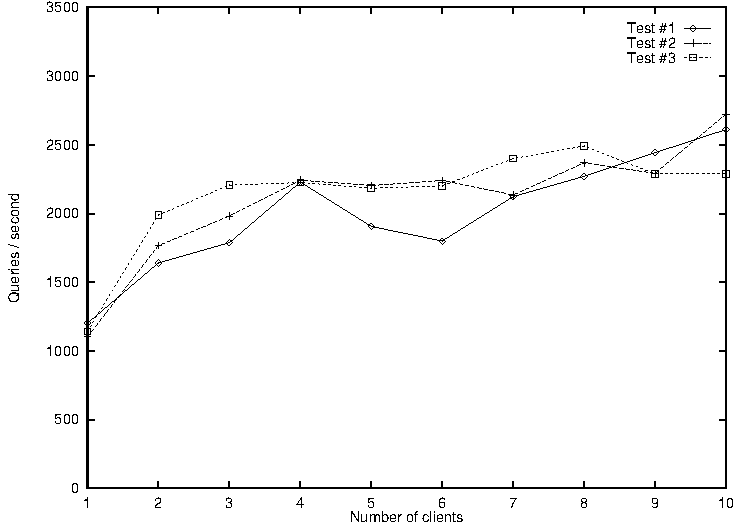
\includegraphics[width=0.9\textwidth]{kuvaesimerkki.pdf}
%\rotatebox{90}{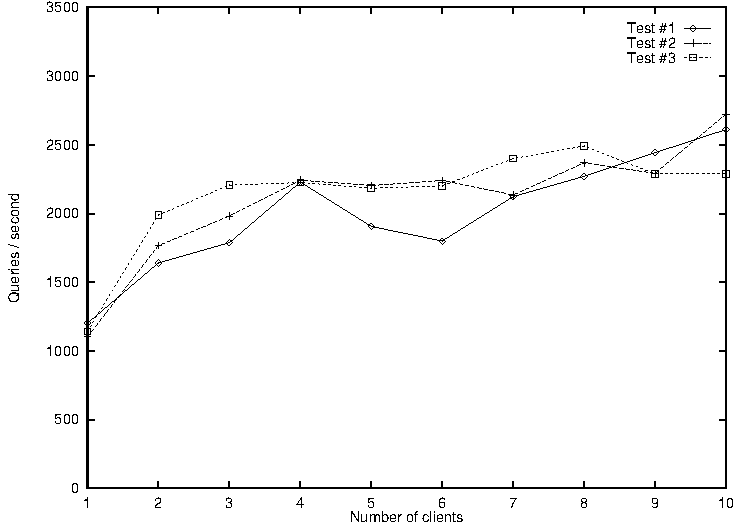
\includegraphics[scale=.75]{kuvaesimerkki.pdf}}
\caption{Figure elements.}
\label{kuvaesimerkki}
\end{center}
\end{figure}


We must also pay attention to the size of figures. Any annotations must be clear and easy to read When 
presenting performance curves, for example, the axels have to be named, the scale notated, and the units 
clearly presented. If you present many things with similar figures, you should use the same scale for easy comparison.

The caption of a figure should be written underneath it, and it is preferable that it be short and to 
the point than too explicit. The same goes for table captions.

Figures and tables should be numbered progressively. In long texts, two-level numbering should be 
used (e.g. Figure 3.1) according to the chapter number, but in shorter texts, one-level numbering is good enough.


You should pay attention to presenting figure and table captions consistently, as well as to punctuation 
marks. It is natural to put a full stop after a caption, since they are most often full sentences. 

(The style for figure and table captions vary according to publisher and publication. The recommendations 
at the Department of Computer Science also seems to vary with respect to where the caption should be placed.)


\section{Headings}

You can use a different font in headings than in the rest of the text, or underlining, larger fonts, or other 
methods of emphasis, but generally it is preferred that you only use one of these methods, because if there are 
very many font types and sizes, the layout looks messy.  The format of headings must be consistent throughout 
the text. You should not use any unnumbered ''extra'' headings.


\section{Using this model}

You can use this text as a model for the layout of your own assignment. The font types and sizes, 
line spacing, etc vary according to word-processing system, so small deviations from the rule are acceptable.

The directive number of pages for written assignments given during the lectures for the Scientific-writing 
course and in this guide are applicable to assignments with a layout like this guide's (font size 12 points). The 
average line in this text should consist of about 80~characters and one page about 30~lines. The number of pages 
includes the text itself and the list of references (the part paginated with Arabic numbers), not the 
cover page, summary, or table of contents.

\chapter{Conclusion}

This text is a checklist for some of the rules governing written presentations, which you should 
keep in mind when writing exercises and theses.

This collection of advise has been compiled by staff members as the
result of discussions on general good writing habbits in computer
science. The consensus is that all young researchers and academic degree
holders must be able to seek and follow instructions of layout and
structuring of texts depending on the contribution they are working on. 
This set of instructions aims at unifying the looks of theses and other
study reports from the department, but it is also a representative of
the instruction sets students will meet later.

This set of instructions only address the looks of the document. Other
instructions must be sought, read and gained experience with in order to
learn to select the suitable semantical contents for the scientific texts.

% MSc instructions
%\chapter{Johdanto}

Seuraavassa on joitain ohjeita tämän tutkielmapohjan käyttöön maisterintutkielmassa. Kirjoittamisohjeita löytyy useasta eri lähteestä. Voit esimerkiksi tutustua kandidaatintutkielman ohjeisiin. 
Ohjaajan kanssa on hyvä keskustella aikaisessa vaiheessa työn rakenteesta.

\chapter{Kuvat ja Taulukot}

\section{Kuvat}
Kuva~\ref{fig:logo} toimii esimerkkinä kuvan lisäämisestä työhön. Muista myös viitata jokaiseen kuvaan tekstissä. 

\begin{figure}[h!] % remove [h!] for automatic placement, which is probalby better for a thesis with more text on page
\centering 

\includegraphics[width=0.3\textwidth]{HY-logo-ml.png}
\caption{Helsingin yliopiston logo matemaattis-luonnontieteellisen tiedekunnan värein.\label{fig:logo}}
\end{figure}

\section{Taulukot}

Taulukossa~\ref{table:results} on esimerkki kokeellisten tulosten raportoinnista taulukkona. Muista myös viitata jokaiseen taulukkoon tekstissä.

\begin{table}[h!]
\centering
\caption{Kokeelliset tulokset.\label{table:results}}
\begin{tabular}{l||l c r} 
Koe & 1 & 2 & 3 \\ 
\hline \hline 
$A$ & 2.5 & 4.7 & -11 \\
$B$ & 8.0 & -3.7 & 12.6 \\
$A+B$ & 10.5 & 1.0 & 1.6 \\
\hline
%
\end{tabular}
\end{table}

\chapter{Viitteet}

\section{Kirjallisuusviitteet}

Kirjallisuuslähteet ylläpidetään erillisessä .bib-tiedostossa. Tässä tutkielmapohjassa käytetyt kirjallisuuslähteet, joista esimerkkejä kuvassa~\ref{bibexamples}, löytyvät tiedostosta\newline \texttt{bibliography.bib}.

\begin{figure}[h!]
    \centering
    \begin{scriptsize}
				
\begin{verbatim}

@article{einstein,
    author =       "Albert Einstein",
    title =        "{Zur Elektrodynamik bewegter K{\"o}rper}. ({German})
        [{On} the electrodynamics of moving bodies]",
    journal =      "Annalen der Physik",
    volume =       "322",
    number =       "10",
    pages =        "891--921",
    year =         "1905",
    DOI =          "http://dx.doi.org/10.1002/andp.19053221004"
}
@book{latexcompanion,
    author    = "Michel Goossens and Frank Mittelbach and Alexander Samarin",
    title     = "The \LaTeX\ Companion",
    year      = "1993",
    publisher = "Addison-Wesley",
    address   = "Reading, Massachusetts"
}
@book{knuth99,
    author    = "Donald E. Knuth",
    title     = "Digital Typography",
    year      = "1999",
    publisher = "The Center for the Study of Language and Information",
    series    = "CLSI Lecture Notes (78)"
}
\end{verbatim}
\end{scriptsize}
    \caption{Esimerkkejä kirjallisuuslähteiden kuvaamisesta .bib-tiedostossa.}
    \label{bibexamples}
\end{figure}

Viitteet kirjallisuuslähteisiin muodostetaan komennolla \texttt{\textbackslash citep\{einstein\}}, josta generoituu tekstiin valitun viittaustyylin mukaisesti muotoiltu viite \citep{einstein}, tai \texttt{\textbackslash citep\{latexcompanion,knuth99\}}, josta tekstiin puolestaan generoituu \citep{latexcompanion,knuth99}. Tekstissä viitatut kirjallisuuslähteet tulevat automaattisesti viiteluetteloon. Kirjallisuuslähteiden tietojen oikeellisuus ja yhdenmukaisuus .bib-tiedostossa vaikuttavat luonnollisesti siihen, miten tiedot tutkielmassa näyttäytyvät. Tämä on syytä huomioida, sillä esim. verkosta valmiiksi {Bib\TeX} muodossa löytyvien tietojen täydellisyyten tai samanmuotoisuuteen ei pidä sokeasti luottaa.  

Keskustele viittaustyylin valinnasta ohjaajan kanssa. Joitain vaihtoehtoja on osoitteessa:\\ 
\url{https://www.overleaf.com/learn/latex/Biblatex_bibliography_styles}.
%\url{https://www.sharelatex.com/learn/Bibtex_bibliography_styles}.

\section{Ristiviitteet}

%Liite~\ref{appendix:model} sivulla~\pageref{appendix:model} sisältää lisämateriaalia.
Taulukossa~\ref{table:results} sivulla~\pageref{table:results} on koottuna kokeelliset tulokset.

% \chapter{Pdf:n luominen tex:stä}

% Linuxissa voit ajaa komentoja \texttt{pdflatex filename.tex} ja \texttt{bibtex filename.tex} vuorotelleen kunnes ohjelmat eivät enää anna varoituksia. Prosessi on helppo automatisoida make-komennon avulla.
 
% \chapter{Johtopäätökset\label{chapter:conclusions}}

% Tutkielma on hyvä päättää johtopäätöksiin tutkielman löydöksistä. 

%\chapter{Introduction}

The following gives some superficial instructions for using this template for a Master's thesis. For guidelines on thesis writing you can consult various sources, for example, the Bachelor thesis template.

The thesis should have an introduction chapter. Other chapters can be named according to the topic. In the end, some summary chapter is needed; see Chapter~\ref{chapter:conclusions} for an example.

\chapter{Figures and Tables}

\section{Figures}
Figure~\ref{fig:logo} gives an example how to add figures to the document. Remember always to cite the figure in the main text.

\begin{figure}[h!] 
\centering 

\includegraphics[width=0.3\textwidth]{HY-logo-ml.png}
\caption{University of Helsinki flame-logo for Faculty of Science.\label{fig:logo}}
\end{figure}

\section{Tables}

Table~\ref{table:results} gives an example how to report experimental results. Remember always to cite the table in the main text. 

\begin{table}
\centering
\caption{Experimental results.\label{table:results}}
\begin{tabular}{l||l c r} 
Experiment & 1 & 2 & 3 \\ 
\hline \hline 
$A$ & 2.5 & 4.7 & -11 \\
$B$ & 8.0 & -3.7 & 12.6 \\
$A+B$ & 10.5 & 1.0 & 1.6 \\
\hline
%
\end{tabular}
\end{table}

\chapter{Citations}

\section{Citations to literature}

References are listed in a separate .bib-file. In this case it is named \texttt{bibliography.bib} including the following content:
\begin{verbatim}
@article{einstein,
    author =       "Albert Einstein",
    title =        "{Zur Elektrodynamik bewegter K{\"o}rper}. ({German})
        [{On} the electrodynamics of moving bodies]",
    journal =      "Annalen der Physik",
    volume =       "322",
    number =       "10",
    pages =        "891--921",
    year =         "1905",
    DOI =          "http://dx.doi.org/10.1002/andp.19053221004"
}
 
@book{latexcompanion,
    author    = "Michel Goossens and Frank Mittelbach and Alexander Samarin",
    title     = "The \LaTeX\ Companion",
    year      = "1993",
    publisher = "Addison-Wesley",
    address   = "Reading, Massachusetts"
}
 
@misc{knuthwebsite,
    author    = "Donald Knuth",
    title     = "Knuth: Computers and Typesetting",
    url       = "http://www-cs-faculty.stanford.edu/%7Eknuth/abcde.html"
}
\end{verbatim}

In the last reference url field the code \verb+%7E+ will translate into \verb+~+ once clicked in the final pdf.

References are created using command \texttt{\textbackslash cite\{einstein\}}, showing as \citep{einstein}. Other examples: \citep{latexcompanion,knuthwebsite}.

Citation style can be negotiated with the supervisor. See some options in \url{https://www.sharelatex.com/learn/Bibtex_bibliography_styles}.

\section{Crossreferences}

Appendix~\ref{appendix:model} on page~\pageref{appendix:model} contains some additional material.

\chapter{From tex to pdf}

In Linux, run \texttt{pdflatex filename.tex} and \texttt{bibtex filename.tex} repeatedly until no more warnings are shown. This process can be automised using make-command.
 
\chapter{Conclusions\label{chapter:conclusions}}

It is good to conclude with a summary of findings. You can also use separate chapter for discussion and future work. These details you can negotiate with your supervisor.


%%%%%%%%%%%%%%%%%%%%%%%%%%%%%%%%%%%%%%%%%%%%%%%%%%%%%%%%%
\cleardoublepage                          %fixes the position of bibliography in bookmarks
\phantomsection
\addcontentsline{toc}{chapter}{\bibname}  % This lines adds the bibliography to the ToC
\printbibliography

%%%%%%%%%%%%%%%%%%%%%%%%%%%%%%%%%%%%%%%%%%%%%%%%%%%%%%%%%
\backmatter
%\begin{appendices}

%
\appendix{Template instructions}


In the HY-CS-main.tex file you will find the following STEPS 0--5. Bellow instructions what each STEP means and how to set up your thesis by following these STEPS.
\vspace{0.5cm}

\textbf{STEP 0 -- Clone the thesis template}

\begin{itemize}
\item One template for all thesis types: \url{https://www.overleaf.com/read/hzgngkgshqwh}
\end{itemize}


{\textbf{STEP 1 -- BSc or MSc thesis?}}
\begin{enumerate}
\item Select whether your are writing BSc (tkt for new, tktl for old) or MSc (csm for new, cs for old, dsm for data science) thesis.
\item Select your language: finnish, english, or swedish.
\item If you are writing MSc select your line / track.
\end{enumerate}


{\textbf{STEP 2 -- Set up your personal information}}

\begin{enumerate}
\item Write the working title of your thesis.
\item Write your name to the author field.
\item Write the names of your supervisors and examiners of the thesis.
\end{enumerate}

{\textbf{STEP 3 -- Write your abstract here}}

\begin{itemize}
\item You can also have the abstract in multiple languages with otherlanguages-environment. Bellow example how to add an english abstract to a thesis written in some other language than english: 

\begin{verbatim}
\begin{otherlanguage}{english} 
\begin{abstract}
Your abstract text goes here. 
\end{abstract} 
\end{otherlanguage}
\end{verbatim}

\end{itemize}

{\textbf{STEP 4 -- Writing your thesis}}

\begin{enumerate}
\item There are some writing instructions in [bsc/msc]\_[finnish/english]\_contents.tex files.
\item You can delete the contents of [bsc/msc]\_[finnish/english]\_contents.tex file and write your thesis inside that file.
\end{enumerate}

{\textbf{STEP 5 -- Set your bibliography style}}

\begin{itemize}
\item The default is Numbering alphabetic order, which should be used in most cases.
\end{itemize}

%
\appendix{Tutkielmapohjan käyttöohjeet}


HY-CS-main.tex tiedosto sisältää viisi askelta STEPS 0--5. Alla on kuvattu, mitä nämä askeleet tarkoittavat ja miten niitä seuraamalla luot itsellesi oikeanlaisen tutkielmapohjan.
\vspace{0.5cm}

\textbf{STEP 0 -- Kopioi itsellesi tutkielmapohja}

\begin{itemize}
\item Tämä sama pohja on käytössä kaikille tutkielmatyypeille:\\ \url{https://www.overleaf.com/read/hzgngkgshqwh}
\end{itemize}


{\textbf{STEP 1 -- BSc vai MSc tutkielma?}}
\begin{enumerate}
\item Valitse (tiedostossa HY-CS-main.tex) oletko tekemässä BSc (tkt uusi tutkinto, tktl vanhatutkinto) vai MSc (csm uusi tutkinto/30~op, cs vanha tutkinto/40~op)
%, dsm datatiede) 
tutkielman.
\item Valitse kieli jolla kirjoitat tutkielman: finnish, english, tai swedish.
\item Jos olet kirjoittamassa MSc tutkielmaa, valitse linja/opintosuunta.
\end{enumerate}


{\textbf{STEP 2 -- Aseta henkilökohtaiset tietosi}}

\begin{enumerate}
\item Kirjoita alustava otsikko tutkielmallesi.
\item Kirjoita oma nimesi.
\item Kirjoita ohjaajien ja tarkastajien nimet (mikäli tiedossa).
\end{enumerate}

{\textbf{STEP 3 -- Kirjoita tiivistelmä(t)}}

\begin{itemize}
\item Voit kirjoittaa tiivistelmän (koko tiivistelmäsivu) eri kielillä \texttt{otherlanguages}-ympäristön avulla. Alla esimerkki jolla kirjoitat englanninkielisen tiivistelmän muulla kuin englannin kielellä kirjoitettuun tutkielmaan:

\begin{verbatim}
\begin{otherlanguage}{english} 
\begin{abstract}
Your abstract text goes here. 
\end{abstract} 
\end{otherlanguage}
\end{verbatim}

\end{itemize}

{\textbf{STEP 4 -- Kirjoita tutkielma}}

\begin{enumerate}
\item Tutkielman kirjoittamista varten löydät ohjeita tiedostosta \newline \texttt{[bsc/msc]\_[finnish/english]\_contents.tex}.
\item Kun olet tutustunut ohjeisiin, voit poistaa tiedoston \newline \texttt{[bsc/msc]\_[finnish/english]\_contents.tex} sisällön ja kirjoittaa oman tutkielmasi kyseiseen tiedostoon.
\end{enumerate}

{\textbf{STEP 5 -- Aseta kirjallisuuslähdeluettelon tyyli}}

\begin{itemize}
\item Oletustyyli tekijä-vuosi, eli (Einstein, 1905), voit vaihtaa tyylin (tiedostossa HY-CS-main.tex) helposti kommentointia muuttamalla numeroituun, eli [1], tai aakkostyyliin, eli [Ein05].
Lisää ohjeita liittyen viittaustyylin säätämiseen {Bib}\TeX issä löytyy verkosta: \url{https://ctan.org/pkg/biblatex}

\end{itemize}


%\appendix{Sample Appendix\label{appendix:model}}
%usually starts on its own page, with the name and number of the appendix at the top. 
%The appendices here are just models of the table of contents and the presentation. Each appendix
%Each appendix is paginated separately.

%In addition to complementing the main document, each appendix is also its own, independent entity.
%This means that an appendix cannot be just an image or a piece of programming, but the appendix must explain its contents and meaning.

%\end{appendices}
%%%%%%%%%%%%%%%%%%%%%%%%%%%%%%%%%%%%%%%%%%%%%%%%%%%%%%%%%

\end{document}
